\documentclass{beamer}

\usepackage{beamerthemesplit}
\usepackage{hyperref}
\usepackage{graphicx}

\newcommand{\ve}[1]{\ensuremath{\mathbf{#1}}}
\newcommand{\vect}[1]{\ensuremath{\mathbf{#1}}}
\newcommand{\ves}[2]{\ensuremath{\mathbf{#1}_\supp{#2}}}
\newcommand{\matr}[1]{\ensuremath{\mathbf{#1}}}
\newcommand{\mats}[2]{\ensuremath{\mathbf{#1}_\supp{#2}}}
\newcommand{\R}{\ensuremath{\mathbb{R}}}
\newcommand{\deriv}[2]{\frac{\partial #1}{\partial #2}}
\newcommand{\mat}[2]{\left(\begin{array}{#1}#2\end{array}\right)}
\newcommand{\brc}[2]{\left\{\begin{array}{#1}#2\end{array}\right.}
\newcommand{\brcs}[1]{\left(#1\right)}

\providecommand\Laplacian{\nabla^2}
\providecommand\bnabla{\boldsymbol{\nabla}}
\providecommand\bLaplacian{\boldsymbol{\nabla}^2}
\providecommand\bV{\boldsymbol{V}}
\providecommand\bx{\boldsymbol{x}}
\providecommand\bz{\boldsymbol{z}}
\providecommand\br{\boldsymbol{r}}
\providecommand\bv{\boldsymbol{v}}
\providecommand\bzhat{\hat{\boldsymbol{z}}}
\providecommand\bnhat{\hat{\boldsymbol{n}}}
\providecommand\brhat{\hat{\boldsymbol{r}}}
\providecommand\btheta{\boldsymbol{\theta}}
\providecommand\bthetahat{\hat{\boldsymbol{\theta}}}
\providecommand\bphi{\boldsymbol{\phi}}
\providecommand\bzero{\boldsymbol{0}}

\title{Computational Electrokinetics}
\author{Roman Zeyde}
\date{\today}

\begin{document}

\frame{\titlepage}

\section*{Outline}
\frame{\frametitle{Outline}\tableofcontents}

\section{Physics}
\subsection{Introduction}
\frame{\frametitle{Colloids and Ion--exchangers}
\begin{itemize}
\item A colloidal system consists of two separate phases:
a dispersed phase (or internal phase) and a continuous phase (or dispersion medium).
\item Electrical double layer phenomenon.
\item Chemical interaction between phases.
\end{itemize}
}
\subsection{Differential Equations}
\frame{\frametitle{Problem Variables}
Dimensionless formulation:
\begin{itemize}
\item $\varphi$ -- electric potential
\item $c_\pm$ -- ionic concentration
\item $\bv$ -- fluid velocity
\item $p$ -- fluid pressure
\end{itemize}
}
\frame{\frametitle{Steady--state equations}
Nernst--Planck equation:
\begin{equation}
\bnabla \cdot (-\bnabla c_\pm \mp c_\pm \bnabla \varphi) + \alpha \bv \cdot \bnabla c = 0
\end{equation}
\[ \bnabla \cdot (\bnabla c + q \bnabla \varphi) = \alpha \bv \cdot \bnabla c \]
\[ \bnabla \cdot (\bnabla q + c \bnabla \varphi) = \alpha \bv \cdot \bnabla q \]
Poisson's equation:
\begin{equation}
\delta^2 \Laplacian \varphi = -q
\end{equation}
Fluid mass conservation:
\begin{equation}
\bnabla \cdot \bv = 0
\end{equation}
Fluid momentum conservation:
\begin{equation}
\bLaplacian \bv - \bnabla p + \Laplacian \varphi \bnabla \varphi = 0
\end{equation}
}
\subsection{Boundary conditions}
\frame{\frametitle{Boundary conditions}
At infinity:
\begin{itemize}
\item Constant electric field: $-\beta \bzhat$.
\item Constant ionic concentration: $C_\infty = 1$.
\item Constant fluid velocity: $\bv = -\mathcal{U} \bzhat$.
\end{itemize}
On the particle:
\begin{itemize}
\item Conductive surface: $\phi = \mathcal{V}$.
\item Constant cationic concentration: $c_+ = \gamma$.
\item Zero anionic flux: $-\bnabla c_- + c_- \bnabla \varphi = \bzero$.
\item No-slip condition: $\bv = \bzero$.
\end{itemize}
In steady state, the particle should be force-free.
}
\frame{\frametitle{Debye layer}
In many realistic scenarios, $\delta \ll 1$ and the majority of the fluid remains electroneutral:
\[q = 0 \Leftrightarrow c_+ = c_-\]
\begin{eqnarray}
\brc{rcl}{\bnabla \cdot (C \bnabla\varPhi) &=& 0 \\
\Laplacian C &=& \alpha \bV \cdot \nabla C \\
\bLaplacian \bV + \Laplacian \varPhi \bnabla \varPhi &=& \bnabla P \\
\bnabla \cdot \bV &=& 0}
\end{eqnarray}
A boundary layer of length $\delta$ is formed near the particle's surface.
The electrokinetic problem can be solved for the inner layer. The solution
can be used as a boundary condition for the outer layer.}
\frame{\frametitle{Bulk scale}
At infinity:
\begin{equation}
\brc{rcl}{\bnabla \varPhi &=& -\beta \bzhat \\ C &=& 1 \\ \bV &=& -\mathcal{U} \bzhat}
\end{equation}
Outside Debye layer:
\begin{equation}
\brc{rcl}{
\varPhi &=& \mathcal{V} - \zeta
\\
\frac{\partial}{\partial n} C &=& C \frac{\partial}{\partial n} \varPhi
\\
\bV &=& \zeta \bnabla_s \varPhi(s) +
2\log\left(1 - \tanh^2 \frac{\zeta}{4}\right) \bnabla_s C
}\end{equation}
Zeta potential:
\begin{eqnarray}
\zeta = \log C - \log \gamma
\end{eqnarray}
}

\subsection{Solutions}
\frame{\frametitle{No applied field$: \beta = 0$}
Static solution:
\begin{eqnarray}
\brc{rcl}{
  \varPhi &=& 0 \\
  C &=&  1 \\
  \bV &=& \bzero \\
  P &=& 0}
\end{eqnarray}
}
\frame{\frametitle{Weak applied field: $\beta \ll 1$}
Result from E. Yariv (2010), ``Migration of ion-exchange particles driven
by a uniform electric field'':
\begin{eqnarray}
\brc{rcl}{
  \varPhi &=& \beta \brcs{\frac{1}{4r^2} - r} \cos\theta \\
  C &=&  1 + \beta\frac{3}{4r^2} \cos\theta \\
  \bV &=& \mathcal{U} \brcs{ \brcs{1 - \frac{a^3}{r^3}} \brhat \cos\theta - \brcs{1 + \frac{a^3}{2r^3}} \bthetahat \sin\theta }\\
  P &=& 0
}
\end{eqnarray}
\begin{eqnarray}
\mathcal{U} = \beta \cdot 2 \log\brcs{\frac{1 + \gamma^{-1/2}}{2}}
\end{eqnarray}

}
\frame{\frametitle{Weak applied field: streamfunction}
\begin{center}
    \includegraphics[width=0.75\textwidth]{coupled_theory.eps}
\end{center}
}

\section{Numerics}
\subsection{Outline}
\frame{\frametitle{Outline}
Laplace: \[\bnabla \cdot (C \bnabla\varPhi) = 0\]
Stokes: \[\brc{rcl}{-\bLaplacian \bV + \bnabla P &=&
    \Laplacian \varPhi \bnabla \varPhi \\
    \bnabla \cdot \bV &=& 0}\]
Advection: \[\Laplacian C - \alpha \bV \cdot \nabla C = 0\]

Iterative relaxation scheme is used.
}
\subsection{Grid selection}
\frame{\frametitle{Grid selection}
\begin{enumerate}
  \item Axisymmetric problem $\rightarrow$ spherical coordinates are used.
  \item Logarithmic grid for $r \in [1, R_\infty]$.
  \item Linear grid for $\theta \in [0 , \pi]$.
  \item Central grid for $C$, $\varPhi$ and $P$.
  \item Staggered grid for $\bV$.
\end{enumerate}
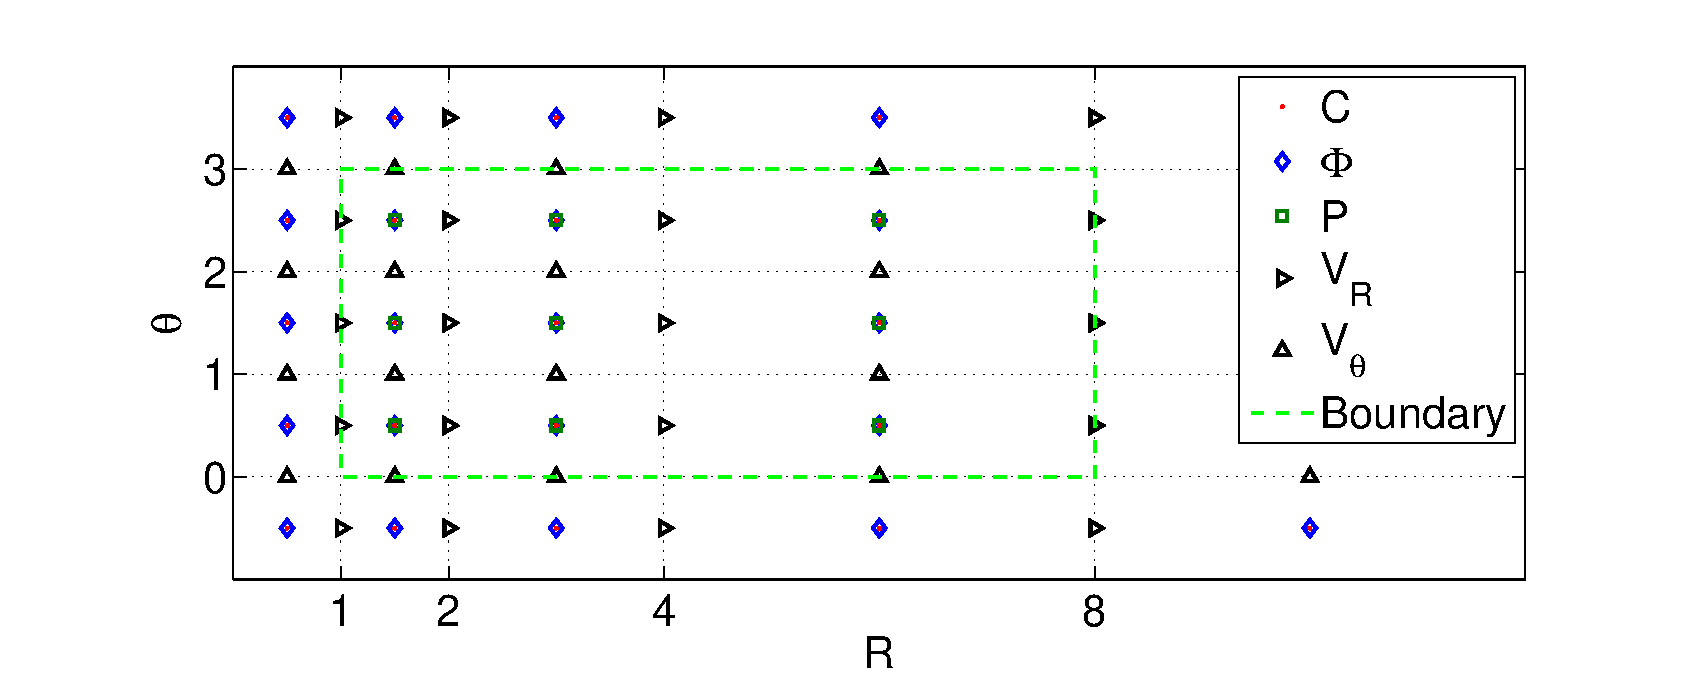
\includegraphics[width=0.75\textwidth]{StaggeredGrid.eps}
}
\subsection{Discretisation}
\frame{\frametitle{Discretisation}
\begin{enumerate}
  \item Each PDE is written as a linear system in one variable, with all other fixed from previous iteration:
      \begin{eqnarray}
        \mathcal{L} u(\bx) = f(\bx)
      \end{eqnarray}
  \item Finite differences method (central/upwind) is used for operator discretisation:
    \begin{eqnarray}
      \sum_j L_{ij} u_j = f_i
    \end{eqnarray}
  \item Dirichlet/Neumann boundary conditions are substituted into the linear system, resulting in $N \times N$ sparse system:
      \begin{eqnarray}
        \matr{A}\vect{u} = \vect{b}
      \end{eqnarray}
      \end{enumerate}
}
\subsection{Iterative solver}
\frame{\frametitle{Iterative solver}
\begin{itemize}
  \item Exact solution of $\matr{A}\vect{u} = \vect{b}$ is too expensive.
  \item Relaxation is applied for each system,
  using preconditioner $\matr{M}$:
  \begin{eqnarray}
    \vect{u}_{n+1} &=& \vect{u}_n + \matr{M}^{-1} \brcs{\vect{b} - \matr{A}\vect{u}_n}
  \end{eqnarray}
  \item $\matr{M}$ should be easy to invert -- O(N) flops.
\end{itemize}
}

\section{Implementation}
\subsection{Spherical coordinates}
\frame{\frametitle{Spherical coordinates}
\begin{itemize}
  \item Gives full symmetry for $\phi$ coordinate: ``2D problem''.
  \item Differential operators' discretisation is more complicated:
  \[\nabla \varPhi, \nabla \cdot \bV, \Laplacian C, \bLaplacian \bV \]
  \item Physics stays invariant under various coordinate systems.
\end{itemize}
}
\subsection{MATLAB sparse matrices}
\frame{\frametitle{MATLAB sparse matrices}}
\subsection{Relaxation}
\frame{\frametitle{Relaxation}} % + acceleration
\subsection{Results}
\frame{\frametitle{Results}
\begin{center}
    \begin{tabular}{cc}
    Convergence of the solver & Comparison to theory \\
    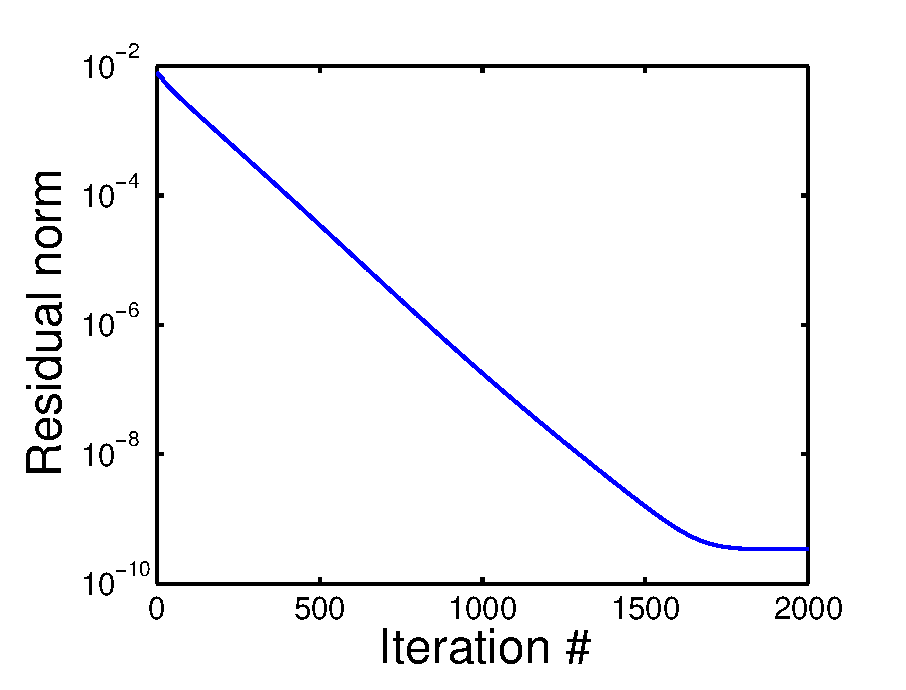
\includegraphics[width=0.5\textwidth]{convergence.eps} &
    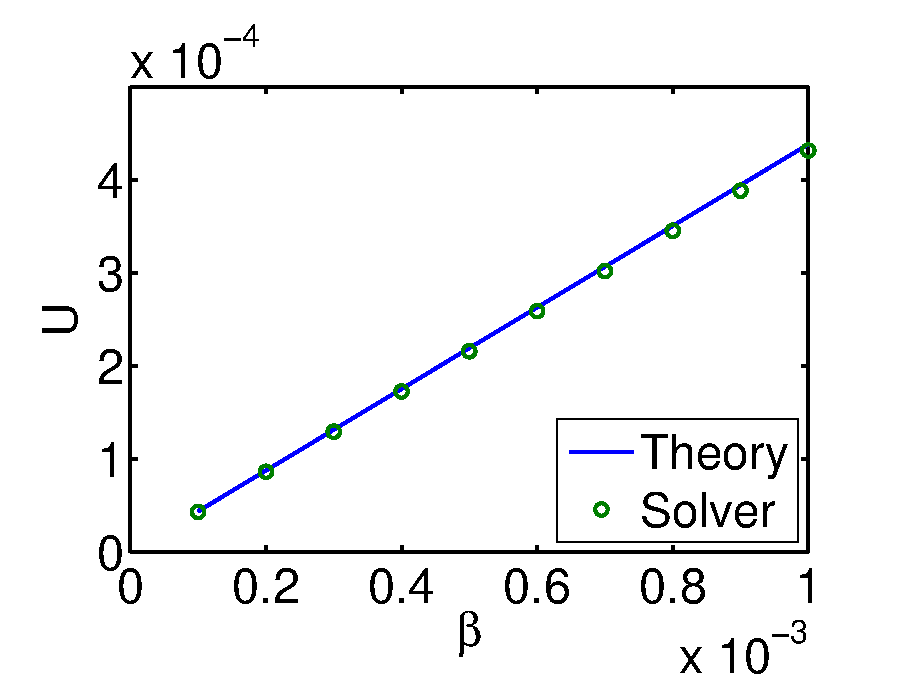
\includegraphics[width=0.5\textwidth]{comparison.eps}
    \end{tabular}
\end{center}}
\frame{\frametitle{Results}
\begin{center}
    \includegraphics[width=0.75\textwidth]{coupled_numeric.eps}
\end{center}}

\end{document}
